% !TeX root=../main.tex
\chapter{مروری بر مطالعات انجام شده}
%\thispagestyle{empty} 
\section{مقدمه}
در این فصل به مرور تعدادی از مقالات مربوط به استراتژی ذخیره‌سازی و سیاست جایگزینی محتوا در حافظه برای شبکه‌های اینترنت اشیا می‌پردازیم. در ادامه الگوریتم‌های استفاده شده در مقالات، معماری به کار رفته برای پیاده‌سازی و چالش‌های آن برای محیط  استفاده شده به طور اجمالی بیان می شوند. 

\section{مروری بر ادبیات موضوع}

\subsubsection{\lr{Caching Transient Content for IoT Sensing: Multi-Agent Soft Actor-Critic}}
	

\begin{figure}[ht]
	\centering 
	\subfloat[روش کنترلی متمرکز]{ \label{fig:centralized}
		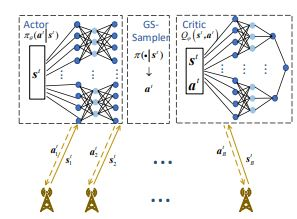
\includegraphics[width=0.4\textwidth]{centralized}}
	\hspace{2mm}
	\subfloat[روش کنترلی غیرمتمرکز]{ \label{fig:decentralized}
		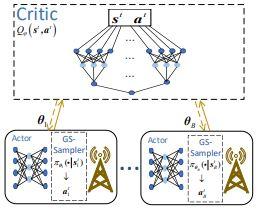
\includegraphics[width=0.4\textwidth]{decntralized}}%
	\caption{دیاگرام الگوریتم \lr{SAC} به کاررفته}
	\label{fig:centralizedvsdec} %% label for entire figure
\end{figure}

\begin{figure}[ht]
	\centerline{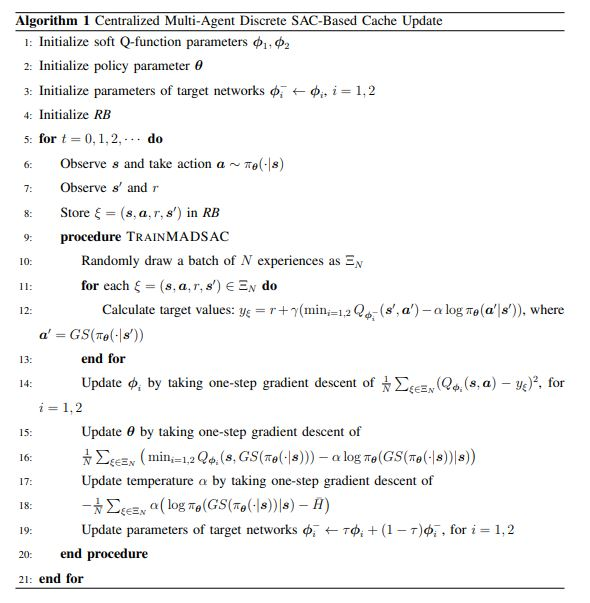
\includegraphics[width=15cm]{centralizedSAC}}
	\caption{الگوریتم \lr{Centralized Soft Actor-Critic}}
	\label{fig:cSACAlgo}
\end{figure}

\begin{figure}[ht]
	\centerline{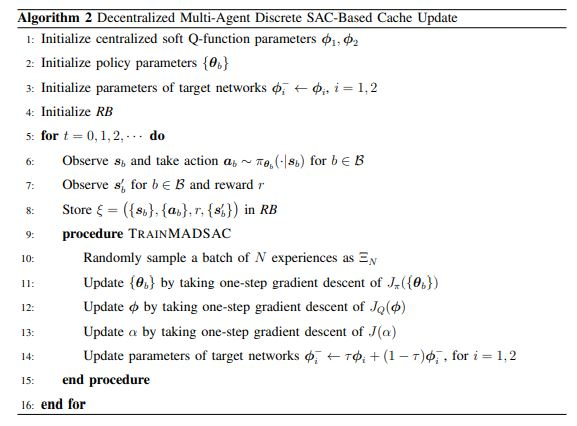
\includegraphics[width=15cm]{decentralizedSAC}}
	\caption{الگوریتم \lr{Decentralized Soft Actor-Critic}}
	\label{fig:dSACAlgo}
\end{figure}

\subsubsection{\lr{Deep Reinforcement Learning for Cooperative Content Caching in Vehicular Edge Computing and Networks}}


\begin{figure}[ht]
	\centerline{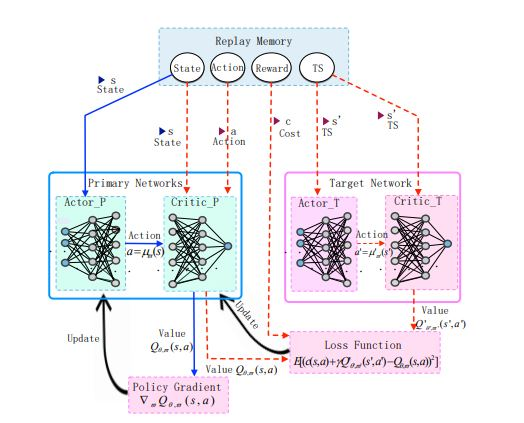
\includegraphics[width=10cm]{PG}}
	\caption{دیاگرام \lr{Deep Deterministic Policy Gradient}}
	\label{fig:PG}
\end{figure}

\begin{figure}[ht]
	\centerline{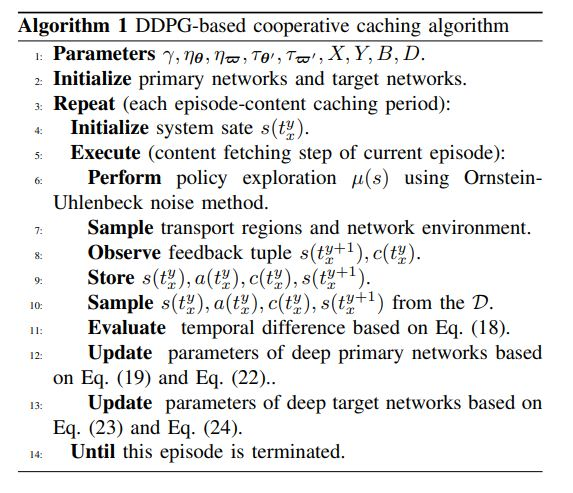
\includegraphics[width=10cm]{DDPG}}
	\caption{الگوریتم \lr{Deep Deterministic Policy Gradient}}
	\label{fig:DDPG}
\end{figure}

\subsubsection{\lr{A Deep Reinforcement Learning-Based Caching Strategy for IoT Networks with Transient Data}}


\begin{figure}[ht]
	\centerline{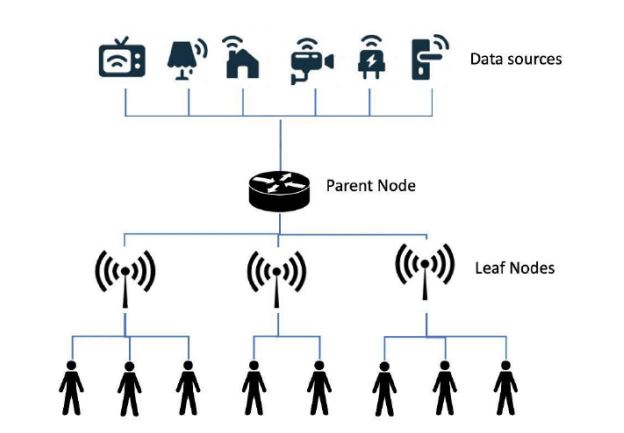
\includegraphics[width=10cm]{parent-leaf}}
	\caption{نمایی از معماری ریشه-برگ}
	\label{fig:parent-leaf}
\end{figure}

\begin{figure}[ht]
	\centerline{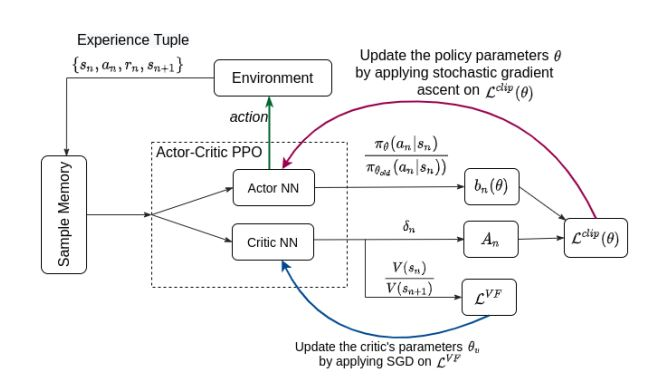
\includegraphics[width=10cm]{PPO-diagram}}
	\caption{دیاگرام \lr{Proximal Policy Optimization}}
	\label{fig:ppod}
\end{figure}

\begin{figure}[ht]
	\centerline{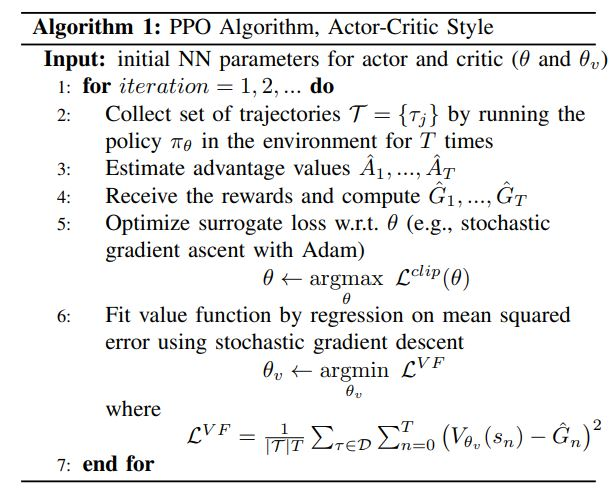
\includegraphics[width=10cm]{PPO}}
	\caption{الگوریتم \lr{Proximal Policy Optimization}}
	\label{fig:ppo}
\end{figure}

\subsubsection{\lr{HFDRL: An Intelligent Dynamic Cooperate Cashing Method Based on Hierarchical Federated Deep Reinforcement Learning in Edge-Enabled IoT}}


\begin{figure}[ht]
	\centerline{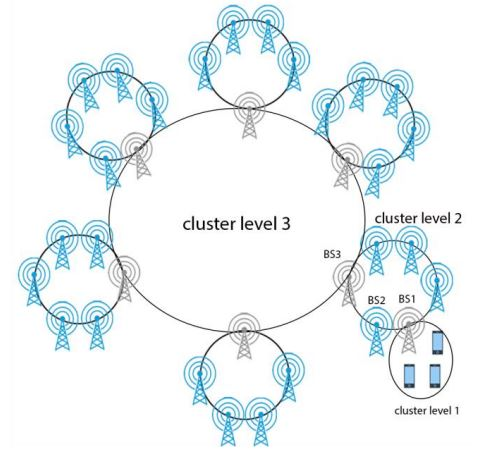
\includegraphics[width=10cm]{cluster-levels}}
	\caption{خوشه‌بندی سه‌لایه‌ای از ایستگاه‌های پایه}
	\label{fig:cluster-levels}
\end{figure}

\begin{figure}[ht]
	\centerline{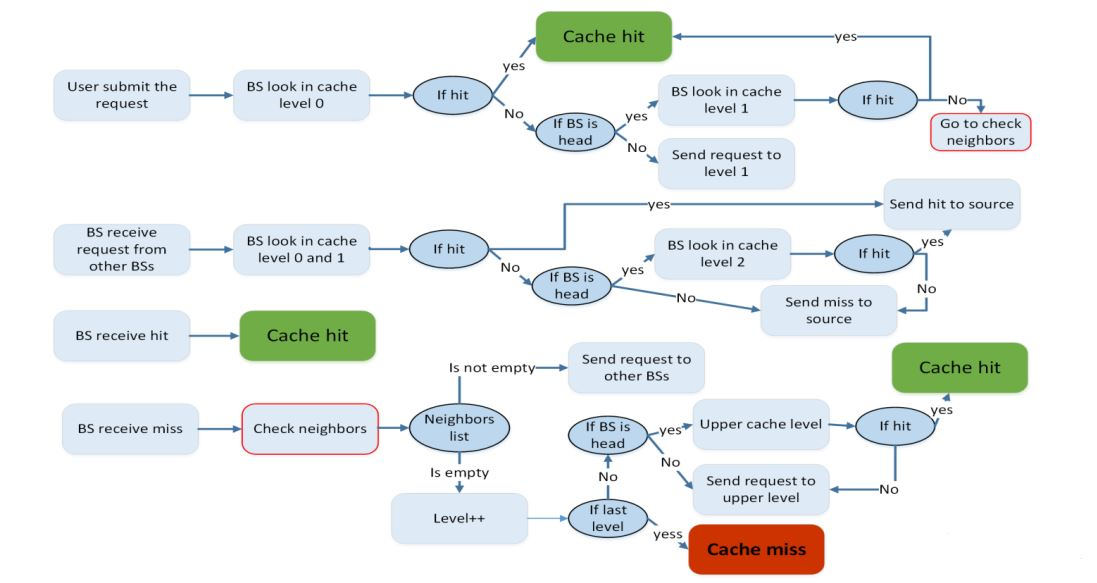
\includegraphics[width=14cm]{FDRL}}
	\caption{دیاگرام جریان داده برای پاسخ به درخواست‌های کاربران در مدل سلسله مراتبی و مشارکتی}
	\label{fig:fdrl}
\end{figure}

\begin{figure}[ht]
	\centerline{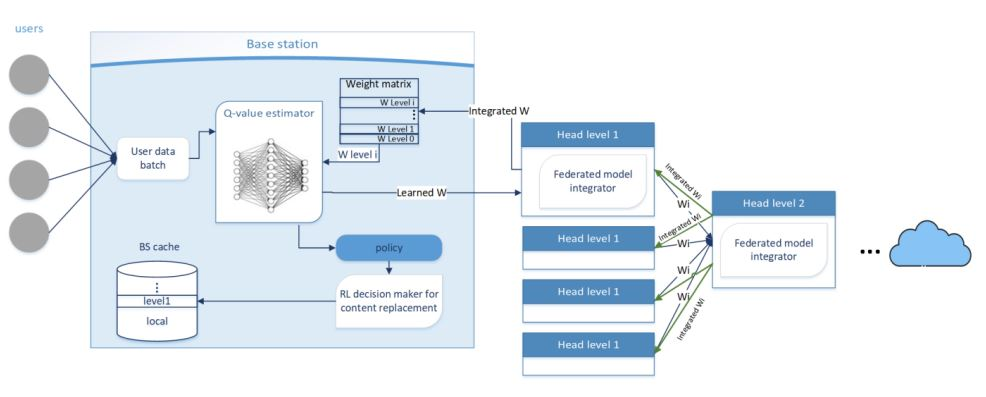
\includegraphics[width=14cm]{HFDRL}}
	\caption{مکانیزم تجمع مدل‌ها در معماری سلسله مراتبی فدراسیونی یادگیری تقویتی عمیق}
	\label{fig:hfdrl}
\end{figure}

